\documentclass{article}
\usepackage[utf8]{inputenc}
\usepackage{graphicx}
\usepackage[hscale = 0.88, vscale = 0.95]{geometry}
\usepackage{hyperref}
\title{Introduction to Chaos Theory}
\date{}

\begin{document}

\maketitle

\section*{Part 1 : Observations from the video.}
Diverse natural phenomena like thermal convection in liquids, neural responses in our brain, the dripping of a faucet, the growth of population of rabbits in an area and the Mandelbrot set all have one aspect in common. This is the logistic equation!
\begin{equation}
        x_{n+1} = rx_n(1-x_n)
\end{equation}
It is a recurrence relation. $r$ is called growth rate. Upon analysis, it has been found that:
\begin{itemize}
    \item For $0<r<1$, the $x_n$ converges to zero, irrespective of the initial value of x.
    \item For $1<r<3$,  $x_n$ converges to some finite value which only depends on r. Irrespective of initial x, it finally converges to this value.
    \item Beyond $r = 3$, interesting things happen. There is no longer an equilibrium value. At first, $x_n$ alternates between two values. As we increase r, it becomes four final values, and then eight, and then after a point, an infinite number of values are taken. It becomes aperiodic, and no value is taken more than once. In this chaotic region, there is sensitive dependence on both r and $x_0$. While these values after large number of iterations depend only on r, these values occur at different iterations based on  $x_0$, and this causes the sensitive dependence in $x_0$ (we had already seen this in our code for logistic map with $r = 3.2$ and different values of $x_0$).  
    \item At some places, there is a reprieve from chaos and stable cycles form again. For any arbitrary period, we can find a corresponding $r$ for which the final cycle follows that period.
\end{itemize}

When these \emph{equilibrium values} are plotted against r, we get the bifurcation diagram. The bifurcation pattern also occurs in the Mandelbrot set. When we see the final value(s) to which the Mandelbrot recurrence converges, we get the bifurcation diagram. One of the main reasons for this is that both the logistic map and the Mandelbrot map are equivalent. Under the linear transformation,
\begin{equation}
    x_n = \frac{-z_n}{r} + \frac{1}{2}
\end{equation}
the logistic map becomes the Mandelbrot map. When we start with $z_0 = 0$ in the Mandelbrot map, it is same as starting from $x_0 = \frac{1}{2}$ in our logistic map.
But this period doubling bifurcations happen in a lot of other places. 
\begin{itemize}
\item The nerve-response system in our brain also seems to follow this pattern when our eye is struck by periodic flickering light.
\item The period doubling is seen in temperature in a fluid with convection due to temperature gradient.
\item The heart rate of a rabbit follows this period doubling pattern during fibrillation. This helps us in knowing when to use electrical shocks to the heart to bring it back to periodicity.
\end{itemize}
\subsection*{Connection to chaos : }
The logistic map is closely related to the chaos theory. A chaotic system is one whose solution is deterministic, but is sensitive to the initial conditions. As a result, even slightly tweaking these initial conditions may result in quite different solutions. \emph{The future predicted by an approximate initial condition may be very different from the actual evolution of the system.}
\subsubsection*{What causes this sensitivity? A detour on phase space}
A phase space is a space which represents all possible  states which a system can take. Every state corresponds to a point in the phase space. Evolution of the system over time results in a \emph{phase space trajectory}. The state can represent anything ranging from position-momentum pair to even $x_n$ in the logistic map. One good aspect which comes from the idea of phase space is that we can now tell "how close" two states are, by numerically computing the Euclidean distance between them. 

Now, lets say that our system is governed by some equation(s). It will have a solution set, where each solution in the set corresponds to one set of initial conditions. Let us think of the following scenarios now :
\begin{itemize}
     \item Consider two "close by" initial states. Let these two states evolve according to the solutions governing them, and lets say we "freeze" the states after letting it evolve for some time. 
     \item If the distance between the states has increased, we tell that our governing equations has \emph{stretched out} the two points.
     \item If the distance between the states has decreased, we tell that our governing equations has \emph{folded} the two points.
\end{itemize}
These stretching and folding operations done by our governing equation is the cause for chaos. 
\begin{itemize}
    \item Stretching results in nearby states going further apart. This results in prediction of future states difficult when we do not know the initial state accurately.
    \item Folding results in considerably far apart states to come close. This makes prediction of the past states inaccurate. Folding also ensures that phase space trajectories are bounded.
\end{itemize}
Stretching and folding mechanisms cloud both the past and the future. 
\subsubsection*{But why is the logistic map chaotic?}
Let us the consider the phase space of $x_n$. The phase space trajectory is an inverted parabola. And this is why it is chaotic! The map is non linear. There is an inherent stretching and folding due to the operations performed by our map. Below is an image illustrating these stretching and folding due to the map. 
\begin{figure}[h]
    \centering{}
    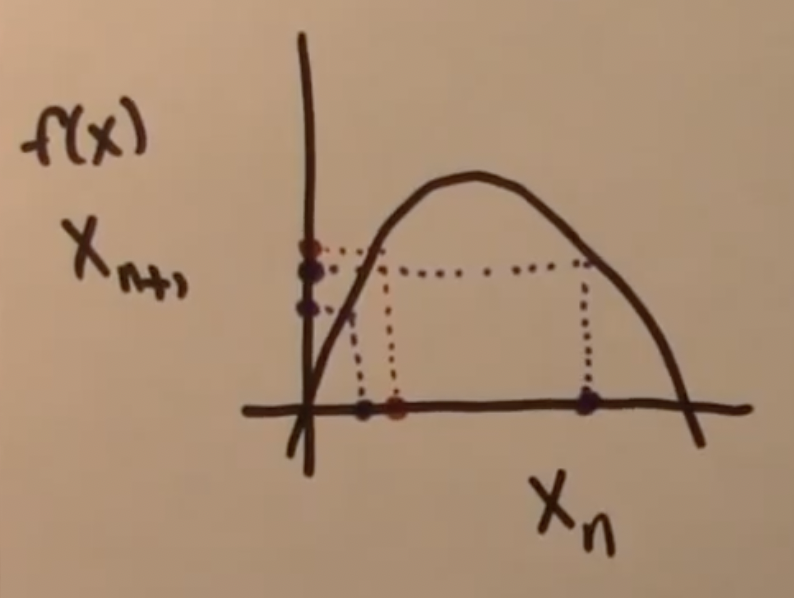
\includegraphics[scale = 0.45]{stretchfold}
\end{figure}
We can see that two nearby $x_n$ results in different $x_{n+1}$, but two values of $x_n$ that are a bit far have nearby $x_{n+1}$.
\section*{Part 2 : Experiments to confirm chaotic behaviors}
Any equation of motion governed by classical mechanics finally boils down to some differential equation(s). Usually, the solution becomes chaotic whenever the number of differential equations increase and/or when there is a non-linear term in the differential equations. While this statement is intuitive and not mathematically rigorous, it gives an idea of when we can expect chaos. 

Note that in the case of logistic map, the system state is discrete and hence represented by a \emph{difference equation(s)} rather than \emph{differential equation(s)} as in continuous state systems.

The following are two simple experiments that can show chaotic behavior.
\subsection*{The double pendulum }
In simple terms, a double pendulum is a pendulum attached to the end of another pendulum. These pendulums can be simple or compound (each is a rigid body). In order to avoid the pendulum colliding on itself, we can perform the experiment with compound pendulum. Upon solving by Lagrangian mechanics, we can see that its governing differential equations are highly non-linear, hence there is sensitive dependence on initial condition. 
\subsubsection*{Resources needed to perform this experiment : }
The resources needed are fairly common and simple too.
\begin{itemize}
    \item Two uniformly dense metal arms with holes at their two ends.
    \item A stand for the double pendulum
    \item Any smooth ball bearing which can connect the two metal arms.
    \item We can also improvise on our experiment. We can take any photo luminescent material as a background, and attach some light source on the free end of our lower metal arm. This would illuminate the path traced by the lowermost point on the photo luminescent material, making the trajectory much clearer.
\end{itemize}
\subsection*{Dynamical billiards : Bunimovich Stadium}
Another fairly simple experiment which is chaotic is the Bunimovich stadium. A stadium is a geometric shape constructed on a rectangle but with semicircles on a pair of opposite sides. Inside the stadium, we let a ball collide with the walls of this stadium. We assume that the collisions are perfectly elastic and that the ball doesn't experience any influence other than collisions i.e it travels in straight lines between successive collisions. The resultant motion is sensitive to initial conditions. Unlike the double pendulum, this doesn't have a differential equation to govern it - only the mechanics of elastic collisions apply. Yet, the system is chaotic. Below is an image illustrating this.

\begin{figure}[h]
    \centering
    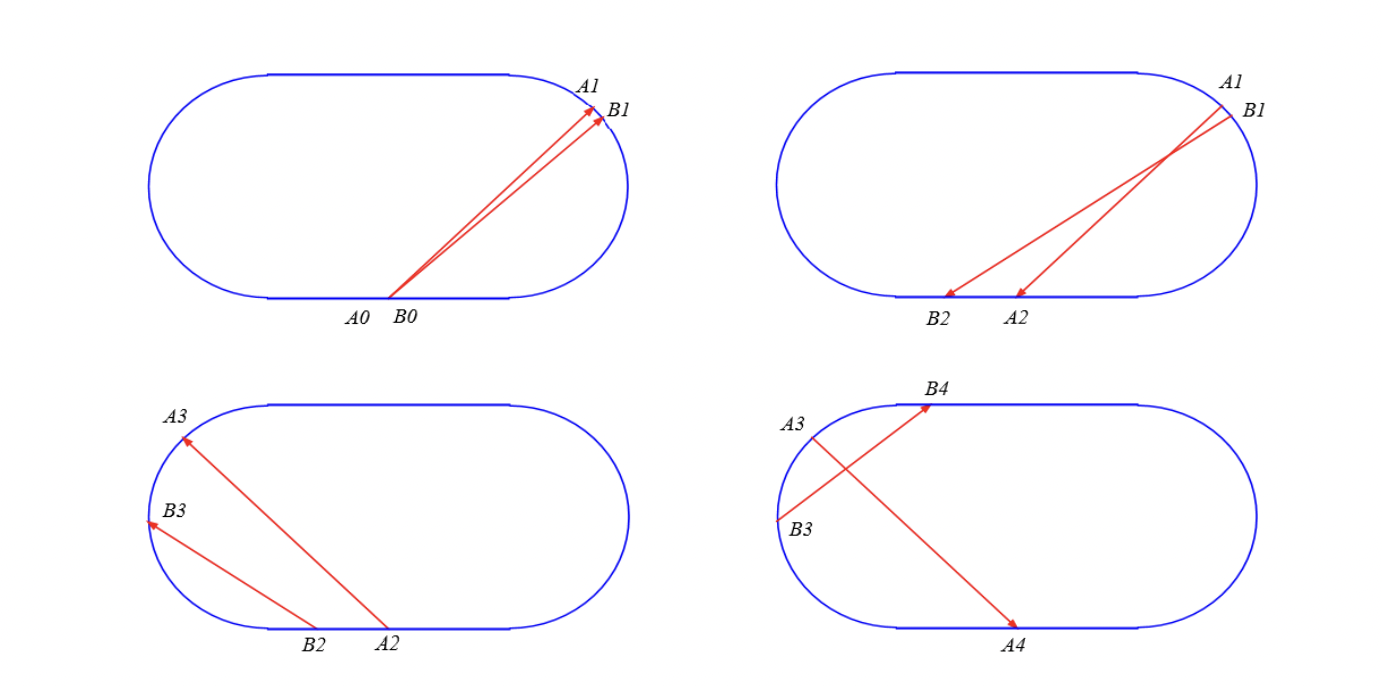
\includegraphics[scale = 0.50]{billiards}
\end{figure}
\subsubsection*{Resources needed to perform this experiment :}
Again, the resources needed are fairly simple. However, we need to ensure that the materials we take have a high coefficient of restitution, so that the collisions are near-elastic. Stainless steel would be one such material.
\begin{itemize}
    \item We would need to construct a stadium. We can try using 3D printing for this.
    \item We need a small ball bearing, which we will collide with the stadium.
    \item A projectile launcher, for launching our ball at a given angle and speed.
    \item We need to eliminate friction. This is not just for energy losses, but the friction can also cause unnecessary rotational motion on the ball. Lubricating the surface can help reduce friction.
\end{itemize}
There are several other interesting variants of this experiment such as putting some charge on our ball and introducing a magnetic field.
\section*{References}

\begin{enumerate}

\item \url{https://geoffboeing.com/2015/04/visualizing-chaos-and-randomness/}

\item \url{https://youtu.be/iDJ6ooKHw_c}

\item \url{https://en.wikipedia.org/wiki/Double_pendulum}

\item \url{https://youtu.be/mZ1hF_-cubA}

\item \url{https://en.wikipedia.org/wiki/Dynamical_billiards}


\end{enumerate}

\end{document}
